\documentclass{beamer}

% Required packages
\usepackage{amsmath}
\usepackage{graphicx}
\usepackage{xcolor}
\usepackage{siunitx}

% Define custom colors for Star Trek DS9 theme
\definecolor{ds9blue}{RGB}{25,25,112}  % Midnight Blue
\definecolor{ds9gold}{RGB}{218,165,32} % Goldenrod
\definecolor{ds9grey}{RGB}{105,105,105} % Dim Gray
\definecolor{ds9red}{RGB}{178,34,34}   % Firebrick

% Set theme
\usetheme{Madrid}

% Customize colors
\setbeamercolor{palette primary}{bg=ds9blue,fg=white}
\setbeamercolor{palette secondary}{bg=ds9grey,fg=white}
\setbeamercolor{palette tertiary}{bg=ds9gold,fg=black}
\setbeamercolor{palette quaternary}{bg=ds9red,fg=white}
\setbeamercolor{structure}{fg=ds9blue}
\setbeamercolor{title}{fg=ds9gold}
\setbeamercolor{subtitle}{fg=ds9gold}
\setbeamercolor{frametitle}{bg=ds9blue,fg=white}
\setbeamercolor{block title}{bg=ds9blue,fg=white}
\setbeamercolor{block body}{bg=ds9grey!20,fg=black}

% Title page configuration
\title[Thermal Physics]{PHYS11 CH:11}
\subtitle{Temperature, Heat, and Phase Changes}
\author[Mr. Gullo]{Mr. Gullo}
\date[March 2025]{March, 2025}
\institute{Physics Department}

\begin{document}

% Title slide
\begin{frame}
    \titlepage
\end{frame}

% Outline slide
\begin{frame}
    \frametitle{Overview}
    \tableofcontents
\end{frame}

% Learning objectives
\begin{frame}
    \frametitle{Learning Objectives}
    \begin{block}{By the end of this lesson, you will be able to:}
        \begin{itemize}
            \item Define temperature and explain its relationship to molecular motion
            \item Convert between temperature scales (Celsius, Fahrenheit, and Kelvin)
            \item Explain the difference between heat and temperature
            \item Calculate heat transfer using $Q = mc\Delta T$
            \item Identify the three mechanisms of heat transfer
            \item Describe phase changes and calculate energy using latent heat
        \end{itemize}
    \end{block}
\end{frame}

\section{Temperature and Thermal Energy}

\begin{frame}
    \frametitle{Temperature and Thermal Energy}
    \begin{columns}
        \column{0.6\textwidth}
        \begin{itemize}
            \item \textbf{Temperature:} Quantity measured by a thermometer
            \item Related to the average kinetic energy of atoms and molecules
            \item \textbf{Absolute zero:} Temperature at which there is no molecular motion
            \item Three main temperature scales:
            \begin{itemize}
                \item Celsius (°C)
                \item Fahrenheit (°F)
                \item Kelvin (K)
            \end{itemize}
        \end{itemize}
        
        \column{0.4\textwidth}
        \begin{center}
            \alert{[Thermometer scales diagram showing comparison of the three temperature scales]}
        \end{center}
    \end{columns}
\end{frame}

\begin{frame}

\begin{figure}
    \centering
    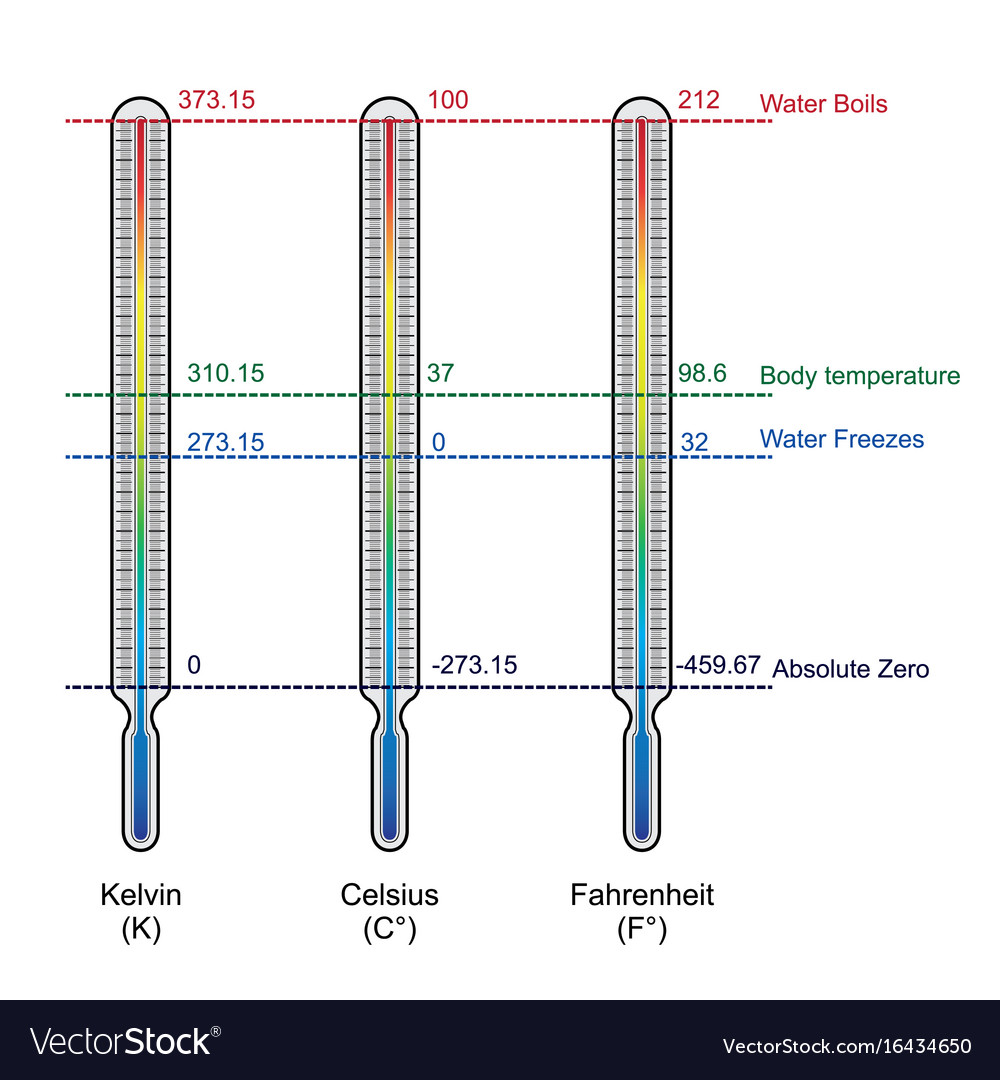
\includegraphics[width=0.75\linewidth]{comparison-three-temperature-scales-vector-16434650-2940992563.jpg}
\end{figure}
\end{frame}


\begin{frame}
    \frametitle{Temperature Scales and Conversion}
    \begin{block}{Temperature Conversion Formulas}
        \begin{align*}
            T_{\text{°F}} &= \frac{9}{5}T_{\text{°C}} + 32 \\
            T_{\text{°C}} &= \frac{5}{9}(T_{\text{°F}} - 32) \\
            T_{\text{K}} &= T_{\text{°C}} + 273.15 \\
            T_{\text{°C}} &= T_{\text{K}} - 273.15
        \end{align*}
    \end{block}
    
    \begin{exampleblock}{Examples}
        \begin{itemize}
            \item Room temperature: $20\text{°C} = 68\text{°F} = 293.15\text{ K}$
            \item Freezing point of water: $0\text{°C} = 32\text{°F} = 273.15\text{ K}$
            \item Absolute zero: $-273.15\text{°C} = -459.67\text{°F} = 0\text{ K}$
        \end{itemize}
    \end{exampleblock}
\end{frame}

\section{Heat, Specific Heat, and Heat Transfer}

\begin{frame}
    \frametitle{Heat and Specific Heat}
    \begin{block}{Definitions}
        \begin{itemize}
            \item \textbf{Heat (Q):} Thermal energy transferred due to a temperature difference
            \item \textbf{Specific heat (c):} Amount of heat needed to raise the temperature of 1 kg of a substance by 1°C
        \end{itemize}
    \end{block}
    
    \begin{alertblock}{Heat Transfer Equation}
        \begin{align*}
            Q = mc\Delta T
        \end{align*}
        where:
        \begin{itemize}
            \item $Q$ = heat transferred (J)
            \item $m$ = mass (kg)
            \item $c$ = specific heat (J/kg·°C)
            \item $\Delta T$ = change in temperature (°C or K)
        \end{itemize}
    \end{alertblock}
\end{frame}

\begin{frame}
    \frametitle{Specific Heat of Common Materials}
    \begin{center}
        \begin{tabular}{|l|c|}
            \hline
            \textbf{Material} & \textbf{Specific Heat (J/kg·°C)} \\
            \hline
            Water & 4,186 \\
            \hline
            Ice (at 0°C) & 2,090 \\
            \hline
            Steam (at 100°C) & 2,010 \\
            \hline
            Aluminum & 900 \\
            \hline
            Copper & 385 \\
            \hline
            Gold & 129 \\
            \hline
            Wood & $\approx$ 1,700 \\
            \hline
        \end{tabular}
    \end{center}
    
    \begin{block}{Note}
        Water has an unusually high specific heat, which is why bodies of water moderate climate.
    \end{block}
\end{frame}

\begin{frame}
    \frametitle{Heat Transfer Methods}
    \begin{columns}
        \column{0.6\textwidth}
        \begin{itemize}
            \item \textbf{Conduction:} Transfer between objects in direct contact
            \begin{itemize}
                \item Metals are good conductors
                \item Wood and air are poor conductors (insulators)
            \end{itemize}
            \item \textbf{Convection:} Transfer by movement of mass
            \begin{itemize}
                \item Ocean currents, boiling water, air movement
            \end{itemize}
            \item \textbf{Radiation:} Transfer by electromagnetic waves
            \begin{itemize}
                \item Requires no medium (works in vacuum)
                \item How the Sun's energy reaches Earth
            \end{itemize}
        \end{itemize}
        
        \column{0.4\textwidth}
        \begin{center}
            \alert{[Diagram showing the three heat transfer mechanisms]}
        \end{center}
    \end{columns}

    \end{frame}

\begin{frame}
\begin{figure}
    \centering
    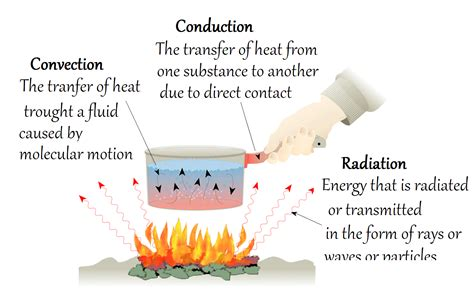
\includegraphics[width=0.75\linewidth]{th-2198955217.jpg}
\end{figure}

\end{frame}



\section{Phase Change and Latent Heat}

\begin{frame}
    \frametitle{Phases of Matter}
    \begin{columns}
        \column{0.55\textwidth}
        \begin{itemize}
            \item Four distinct phases:
            \begin{itemize}
                \item \textbf{Solid:} Particles in fixed positions, vibrating
                \item \textbf{Liquid:} Particles close together but can move around
                \item \textbf{Gas:} Particles far apart, moving freely
                \item \textbf{Plasma:} Ionized gas (very high energy)
            \end{itemize}
            \item Gas is the most energetic state
            \item Solid is the least energetic state
        \end{itemize}
        
        \column{0.45\textwidth}
        \begin{center}
            \alert{[Phase transition diagram showing the four states of matter and the energy relationships between them]}
        \end{center}
    \end{columns}
\end{frame}

\begin{frame}
\begin{figure}
    \centering
    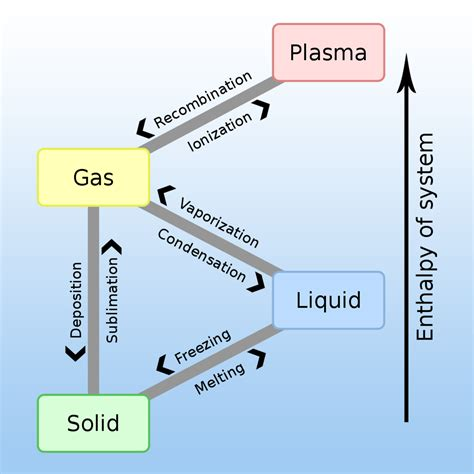
\includegraphics[width=0.75\linewidth]{th-1470353042.jpg}
\end{figure}
\end{frame}




\begin{frame}
    \frametitle{Phase Changes}
    \begin{columns}
        \column{0.5\textwidth}
        \begin{itemize}
            \item \textbf{Melting:} Solid → Liquid
            \item \textbf{Freezing:} Liquid → Solid
            \item \textbf{Vaporization:} Liquid → Gas
            \item \textbf{Condensation:} Gas → Liquid
            \item \textbf{Sublimation:} Solid → Gas
            \item \textbf{Deposition:} Gas → Solid
        \end{itemize}
        
        \column{0.5\textwidth}
        \begin{block}{Important Points}
            \begin{itemize}
                \item Phase changes occur at fixed temperatures
                \item No temperature change during phase change
                \item Energy breaks bonds between particles
                \item Increases potential energy, not kinetic energy
            \end{itemize}
        \end{block}
    \end{columns}
\end{frame}

\begin{frame}
    \frametitle{Latent Heat}
    \begin{block}{Definition}
        \textbf{Latent heat:} The energy required to change the phase of a substance without changing its temperature
    \end{block}
    
    \begin{alertblock}{Heat Transfer Equations for Phase Changes}
        \begin{align*}
            Q_{\text{melting/freezing}} &= mL_f \\
            Q_{\text{vaporization/condensation}} &= mL_v
        \end{align*}
        where:
        \begin{itemize}
            \item $Q$ = heat transferred (J)
            \item $m$ = mass (kg)
            \item $L_f$ = latent heat of fusion (J/kg)
            \item $L_v$ = latent heat of vaporization (J/kg)
        \end{itemize}
    \end{alertblock}
\end{frame}

\begin{frame}
    \frametitle{Latent Heat Values}
    \begin{center}
        \begin{tabular}{|l|c|c|}
            \hline
            \textbf{Substance} & \textbf{Latent Heat of Fusion (kJ/kg)} & \textbf{Latent Heat of Vaporization (kJ/kg)} \\
            \hline
            Water & 334 & 2,260 \\
            \hline
            Aluminum & 380 & 11,400 \\
            \hline
            Gold & 64.5 & 1,580 \\
            \hline
            Mercury & 11.8 & 296 \\
            \hline
            Tungsten & 184 & 4,810 \\
            \hline
        \end{tabular}
    \end{center}
    
    \begin{block}{Note}
        During phase changes, the temperature remains constant while energy is being added or removed.
    \end{block}
\end{frame}

\section{Examples and Applications}

\begin{frame}
    \frametitle{"I do" Example}
    \begin{block}{Problem}
        How much energy would it take to heat 1.00 kg of ice at 0°C to water at 15.0°C?
    \end{block}
    \end{frame}

\begin{frame}
    \begin{exampleblock}{Solution}
        \begin{enumerate}
            \item Energy to melt ice at 0°C to water at 0°C:
            \begin{align*}
                Q_1 &= mL_f = 1.00 \text{ kg} \times 334 \text{ kJ/kg} = 334 \text{ kJ}
            \end{align*}
            
            \item Energy to heat water from 0°C to 15.0°C:
            \begin{align*}
                Q_2 &= mc\Delta T\\
                &= 1.00 \text{ kg} \times 4,186 \text{ J/(kg·°C)} \times 15.0 \text{ °C}\\
                &= 62,790 \text{ J} = 62.8 \text{ kJ}
            \end{align*}
            
            \item Total energy required:
            \begin{align*}
                Q_{\text{total}} &= Q_1 + Q_2 = 334 \text{ kJ} + 62.8 \text{ kJ} = 397 \text{ kJ}
            \end{align*}
        \end{enumerate}
    \end{exampleblock}
\end{frame}

\begin{frame}
    \frametitle{"We do" Example}
    \begin{block}{Problem}
        Ice cubes are used to chill a soda with a mass of 0.250 kg at 15.0°C. The ice is at 0°C, and the total mass of the ice cubes is 0.020 kg. Assume that the soda is kept in a foam container so that heat loss can be ignored, and that the soda has the same specific heat as water. Find the final temperature when all ice has melted.
    \end{block}
    
    \begin{exampleblock}{Solution Steps}
        \begin{enumerate}
            \item Heat lost by soda = Heat gained by ice
            \item Heat lost by soda: $Q_{\text{soda}} = m_{\text{soda}}c_{\text{water}}(T_f - T_i)$
            \item Heat gained by ice: $Q_{\text{ice}} = m_{\text{ice}}L_f + m_{\text{ice}}c_{\text{water}}(T_f - 0\text{°C})$
            \item Set $Q_{\text{soda}} = Q_{\text{ice}}$ and solve for $T_f$
            \item $T_f = 9.03\text{°C}$
        \end{enumerate}
    \end{exampleblock}
    
\end{frame}

\begin{frame}
    \frametitle{"You do" Example}
    \begin{block}{Problem}
        A certain quantity of water is given 4.0 kJ of heat. This raises its temperature by 30.0°F. What is the mass of the water in grams?
    \end{block}
    
    \begin{alertblock}{Hints}
        \begin{itemize}
            \item Use the equation $Q = mc\Delta T$
            \item Remember to convert temperature change from °F to °C
            \item The specific heat of water is 4,186 J/(kg·°C)
        \end{itemize}
    \end{alertblock}
    
    Take some time to work this out. Then we'll discuss the solution.
    
    \pause
    
    \begin{exampleblock}{Answer}
        The mass of water is 57 g.
    \end{exampleblock}
\end{frame}

\section{Summary}

\begin{frame}
    \frametitle{Key Equations}
    \begin{columns}
        \column{0.5\textwidth}
        \textbf{Temperature Conversions:}
        \begin{align*}
            T_{\text{°F}} &= \frac{9}{5}T_{\text{°C}} + 32 \\
            T_{\text{°C}} &= \frac{5}{9}(T_{\text{°F}} - 32) \\
            T_{\text{K}} &= T_{\text{°C}} + 273.15
        \end{align*}
        
        \column{0.5\textwidth}
        \textbf{Heat Transfer:}
        \begin{align*}
            Q &= mc\Delta T \\
            Q_{\text{melting/freezing}} &= mL_f \\
            Q_{\text{vaporization/condensation}} &= mL_v
        \end{align*}
    \end{columns}
\end{frame}

\begin{frame}
    \frametitle{Summary}
    \begin{block}{Temperature and Thermal Energy}
        \begin{itemize}
            \item Temperature relates to average kinetic energy of particles
            \item Three main scales: Celsius, Fahrenheit, Kelvin
            \item Absolute zero: no molecular motion
        \end{itemize}
    \end{block}
    
    \begin{block}{Heat, Specific Heat, and Heat Transfer}
        \begin{itemize}
            \item Heat is energy transfer due to temperature difference
            \item $Q = mc\Delta T$ relates heat, mass, specific heat, and temperature change
            \item Heat transfer methods: conduction, convection, radiation
        \end{itemize}
    \end{block}
    
    \begin{block}{Phase Change and Latent Heat}
        \begin{itemize}
            \item Four phases: solid, liquid, gas, plasma
            \item Phase changes occur at constant temperature
            \item Heat added during melting/vaporization, released during freezing/condensation
        \end{itemize}
    \end{block}
\end{frame}

\begin{frame}
    \frametitle{Thank You!}
    \begin{center}
        \Huge{Questions?}
        
        \vspace{1cm}
        \normalsize
        Remember to review the key equations and concepts for the upcoming quiz!
    \end{center}
\end{frame}

\end{document}